\section{Non-parametric: Meanshift}

\subsection{What?}
\subsubsection{Clustering and Modes of Probability Density Function}
Mean shift  is a popular non-parametric clustering algorithm based on the
idea of associating each data point to a mode of the underlying probability density
function\textsuperscript{2.1}.Meanshift is a powerful tool for us in this case although the idea behind it is very simple. {\linebreak}

Assuming that we have a dataset of students and corresponding mark for each of them 
in final exam as the table below. How do we categorize these students into groups (clustering) base on their marks?
\begin{center}
 \begin{tabular}{||c c c||} 
 \hline
 No & Student & Mark \\ [0.5ex] 
 \hline\hline
 1 & S1 & 5.0 \\ 
 \hline
 2 & S2 & 4.0 \\
 \hline
 3 & S3 & 4.5 \\
 \hline
 4 & S4 & 5.7 \\
 \hline
 5 & S5 & 6.0 \\ 
  \hline
 6 & S6 & 9.0 \\ 
  \hline
 7 & S7 & 8.7 \\ 
  \hline
 8 & S8 & 9.5 \\ 
 [1ex] 
 \hline
\end{tabular}
\end{center}

Imagine that the set of marks was sampled from a probability distribution. We seek for the modes of  the underlying distribution for this set of marks. Number of modes corresponds to the number of groups of students.
\pgfplotsset{grid style={dashed,gray}}
\pgfplotsset{minor grid style={dashed,red}}
\pgfplotsset{major grid style={dotted,green!50!black}}

%Probability plot
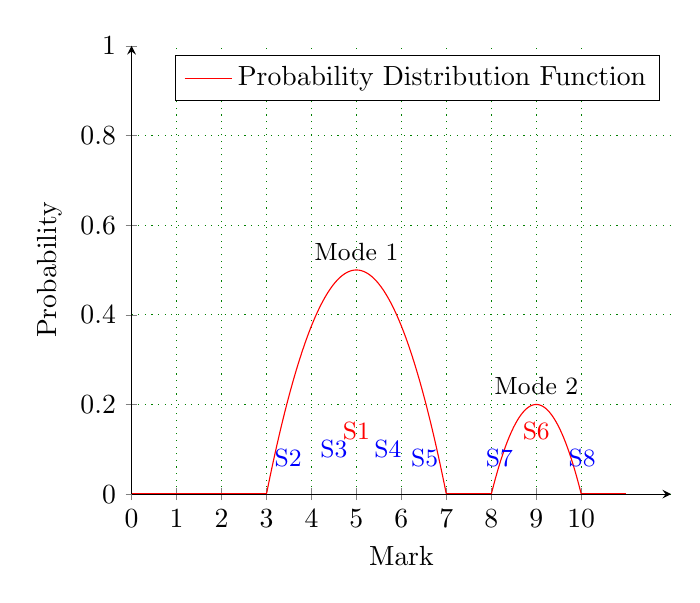
\begin{tikzpicture}
	\begin{axis}[
	axis lines=left,
	xtick={0,1,...,10},ytick = {0,0.2,...,1},
	grid=both,
	xlabel = {Mark},
	ylabel = {Probability}
	]
		%First Mode
		\addplot [
		domain=3:7,
		samples=100,
		color=red,
		]
		{-0.125*x^2 + 1.25*x - 2.625};
		
		\addplot [
		 domain=0:3,
		 samples=10, 
		 color=red,
		 ]
		 {0.002};
		 \addplot [
		 domain=7:8,
		 samples=10, 
		 color=red,
		 ]
		 {0.002};
		 \addplot [
		 domain=10:11,
		 samples=10, 
		 color=red,
		 ]
		 {0.002};
		 \addplot [
		domain=0:12, 
		samples=2,
		color = white
		]
		{1};
		%Second mode
		\addplot [
		domain=8:10, 
		samples=100, 
		color=red,
		]
		{-0.2*x^2 + 3.6*x - 16};
		 
		 %First Mode
		
		\draw[red,fill,thick] (50,50) circle (0.05cm);
		\node[black,above] at (axis cs:5,0.5){\small{Mode 1}};
		 %S1
		\draw[red,thick] (50,4) circle (0.2cm);
		\node[red,above] at (axis cs:5,0.1){\small{S1}};
		 %S2
		\draw[blue,thick] (40,4) circle (0.2cm);
		\node[blue,left] at (axis cs:4,0.08){\small{S2}};
		 %S3
		\draw[blue,thick] (45,4) circle (0.2cm);
		\node[blue,above] at (axis cs:4.5,0.06){\small{S3}};
		 %S4
		\draw[blue,thick] (57,4) circle (0.2cm);
		\node[blue,above] at (axis cs:5.7,0.06){\small{S4}};
		 %S5
		\draw[blue,thick] (60,4) circle (0.2cm);
		\node[blue,right] at (axis cs:6,0.08){\small{S5}};
		
		 %Second Mode
		 
		 \draw[red,fill,thick] (90,20) circle (0.05cm);
		 \node[black,above] at (axis cs:9,0.2){\small{Mode 2}};
		 %S6
		\draw[red,thick] (90,4) circle (0.2cm);
		\node[red,above] at (axis cs:9,0.1){\small{S6}};
		 %S7
		\draw[blue,thick] (87,4) circle (0.2cm);
		\node[blue,left] at (axis cs:8.7,0.08){\small{S7}};
		 %S8
		\draw[blue,thick] (95,4) circle (0.2cm);
		\node[blue,right] at (axis cs:9.5,0.08){\small{S8}};
		
		%Legend
		\addlegendentry{Probability Distribution Function}
	\end{axis}
\end{tikzpicture}

As can be seen from the graph above, we have two groups of students correspond to two modes of probability distribution function. 
With Mode 1, we have first group which includes: S1, S2, S3, S4, S5.  Similarly, correspoding to Mode 2 is second group, which includes : S6, S7, S8. That's why we can use mode-seeking algorithms as a solution of Clustering problem.
\subsubsection{Gradient Ascent and Modes of Probability Density Function}
The Taylor series of a function f(x) is described by the equation \textsuperscript{[2.2]}:
\[
    f(x+a) = f(x) + \frac{f'(x)}{1!}a+\frac{f''(x)}{2!}a^2+\frac{f'''(x)}{3!}a^3+...+\frac{f^{(n)}(x)}{n!}a^n
\]
\[\Longrightarrow f(x+a) \approx f(x) + \frac{f'(x)}{1!}a =  f(x) + f'(x)a\]
with a: learning rate,  f'(x): derivative or gradient of f(x)\\
Back to previous example in 3.1.1, let's say f(x) is the probability distribution function. As the illustration of the below graph, from any point on the graph of f(x), we continously move a small step f'(x).a$>$0 (Gradient Ascent) until reaching a local mode of f(x).\\ 
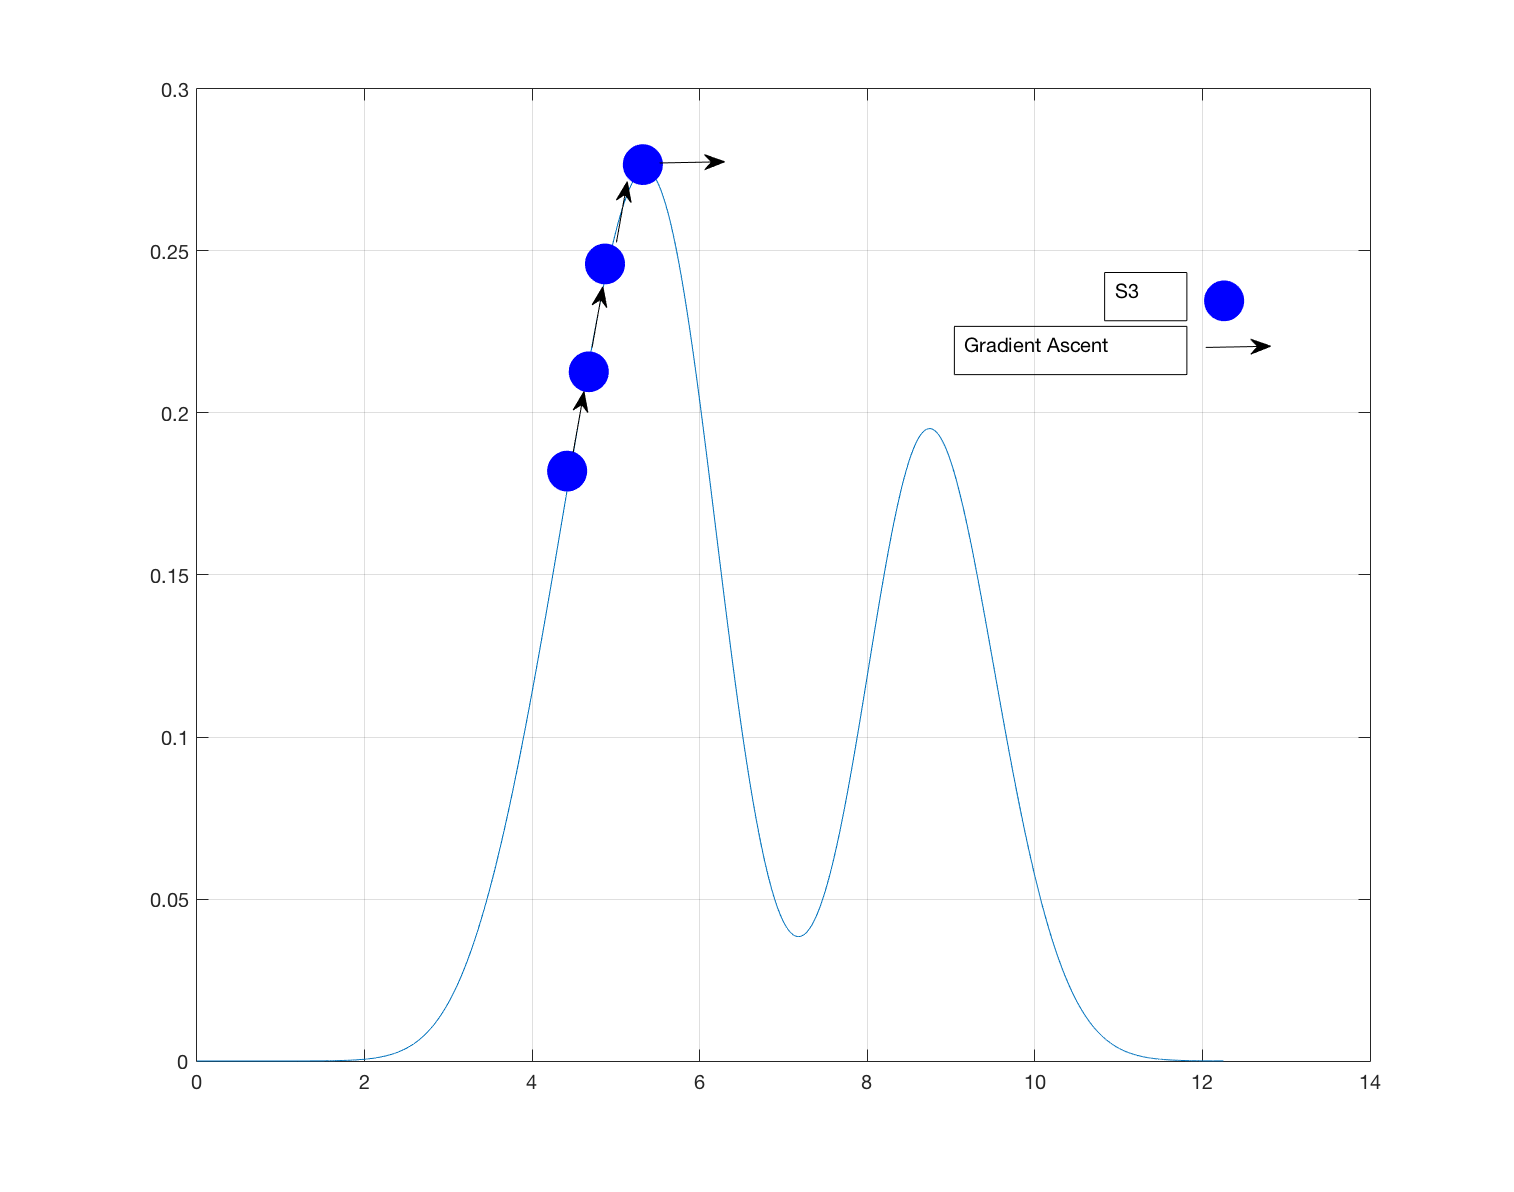
\includegraphics[width=\textwidth]{gradientAscent}
Important result: We can find modes of a probability density function by shifting a proper gradient ascent step from any point of that function.
The pseudo code for Gradient Ascent algorithm:\\
Repeat until convergence: \{\\
f(x) := f(x) + f'(x)a;\\
\}
\subsubsection{Meanshift and Gradient Ascent}

According to Domaniciu with given n data points x\textsubscript{i} i = 1,...,n in the d-dimensional space R\textsuperscript{d}, the multivariate kernel density estimator (Probability Density Function) is f(x) and the mean shift vector of f(x) is defined as:
	%\[f(x) = \frac{1}{n}\sum_{i=1}^{n}K_H(x-x_i)\]
	%(\norm{\vb{\frac{x-x_i}{h}}}^2})
	\[m(x) = \frac{\sum_{i=1}^{n}x_i{w(x_i) }}{\sum_{i=1}^{n}{w(x_i) }) }-x\]
Domaniciu also shows that m(x) is propotional to the gradient of f(x):$\nabla$f(x). This is the keypoint of mean
\subsection{Why?}

\subsection{How?}

\subsection{Advantages and disadvantages}

2.2 https://web.stanford.edu/class/cs168/l/l5.pdf